% DO NOT COMPILE THIS FILE!! It contains snippet of TeX code that may
% be useful when writing an article, or whatever...

%%% EPIGRAPH 
% - preamble
\usepackage{epigraph}                                      % for inspirational quotes...
\setlength{\epigraphwidth}{0.8\columnwidth}                % ... with the right length...
% - code
\section{Some section}
  \epigraph{\emph{Ah, the beauty of math!}}{Yours Truly}

%%% ENDNOTES
% - preamble
\usepackage{endnotes}
\renewcommand{\theendnote}{\Roman{endnote}}                % make endnotes use roman numbers, to distinguish them from footnotes (which use arabic numbers)
% - code to create an endnote
\endnote{This is an example endnote}
% --- code to show endnotes ---
\begingroup
\addcontentsline{toc}{section}{Notes}
\renewcommand{\enotesize}{\small}
%\def\enoteheading{\section*{Notas}}   % if you need to change the Note's %section title
\theendnotes
\endgroup
% --- end endnotes ---

% MATH SPACING
For spacing: In a ``math'' environment, LaTeX ignores the spaces you type and 
puts in the spacing that it thinks is best. LaTeX formats mathematics the
way it’s done in mathematics texts. If you want different spacing, LaTeX 
provides the following four commands for use in math mode: 

\begin{verbatim}
\; - a thick space

\: – a medium space

\, – a thin space

\! – a negative thin space 
  \end{verbatim}

\section{Graphics}
  % image source: 
  % http://tumblring.net/wp-content/uploads/2011/01/tumblr-tumbeasts.png
  \begin{figure}[ht!]
    \centering
    %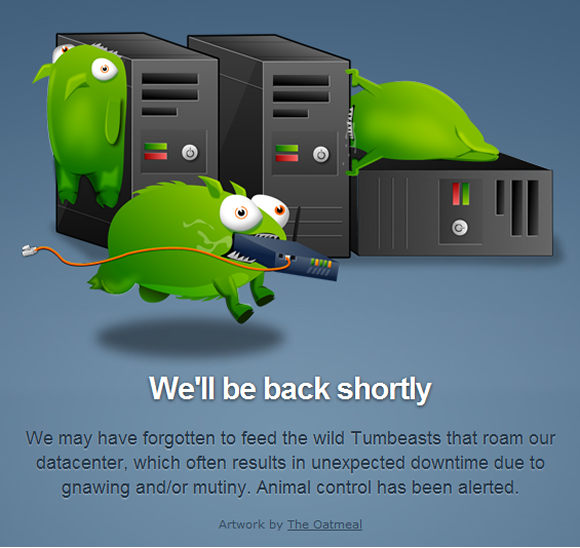
\includegraphics{tumbeasts.jpg}
    %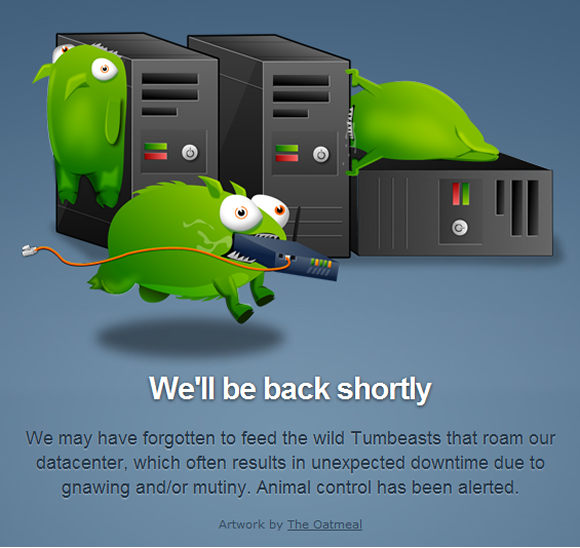
\includegraphics[width=0.5\columnwidth]{tumbeasts.png}
    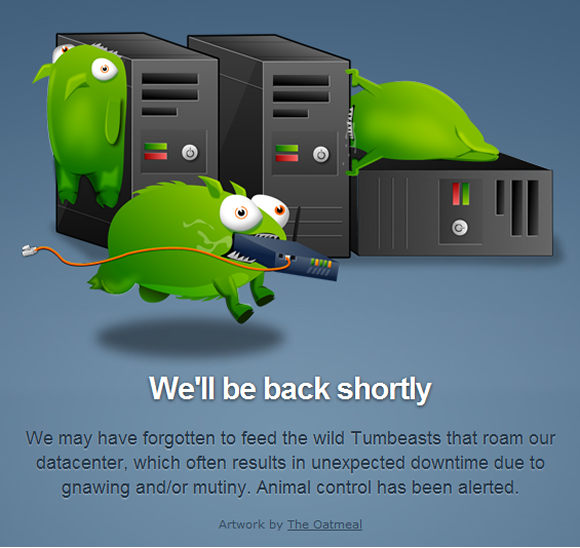
\includegraphics[scale=0.42]{tumbeasts.png}
    \caption{A simple caption}
    \label{overflow}
  \end{figure}

% for ``articles'' for which you need a custom signature
% must be used in one-column mode only! (and at the end of the body)
\begin{minipage}[c]{\textwidth}
  \vspace{1cm}
  \flushright\parbox{7.5cm}{\emph{Yours sincerely}\\
  \\[1.0cm]
  Yours Truly's Full Name}
  \flushright\parbox{7.5cm}{}
  \vspace{1cm}
\end{minipage}

\section{Styles, et al.}
  Here I'll describe a way of installing \LaTeX\ styles, BiBTeX styles, and a couple 
  of other things in a straightforward way---I think this should work with most 
  *nix systems.

  The first thing to do, is discover where whatever you want to install should 
  be installed. And the ideal way to do this is using a tool named kpsewhich, 
  which should get installed when you install LaTeX. It can be used to do a lot 
  of things (\verb+$ kpsewhich --help+), but the one we’re interested in here, 
  location of styles, uses the \verb+--show-path NAME+ option. The list of 
  allowed names is part of the output of the \verb+--help+ option. So for 
  instance, to discover where to place BiBTeX style files (*.bst), run:
  \begin{verbatim}
kpsewhich --show-path bst
  \end{verbatim}

  This will output a list of locations where BiBTeX style files are searched 
  for. So if you have a file called mystyle.bst, create a folder named 
  ``mystyle" in the appropriate location (I use 
  \verb+/home/user/texmf/bibtex/bst/+), and put mystyle.bst inside the folder 
  you just created. Then run \verb+$ texhash .+ (don’t forget the dot!) from the 
  ``appropriate location'' folder you used. And you're done!
